\documentclass[12pt]{article}
\usepackage{scrtime} % for \thistime (this package MUST be listed first!)
\usepackage[margin=0.75in]{geometry}
\usepackage{graphicx}
\usepackage{fancyhdr}
\usepackage{caption}
\usepackage{subcaption}
\usepackage{xspace}
\usepackage[colorlinks]{hyperref} %urls and hyperlinks
%change colour of the links
\hypersetup{
	colorlinks,
	linkcolor={black},
	citecolor={blue!50!black},
	urlcolor={blue}
}
%\usepackage{underscore}
\usepackage{pdfpages}
\usepackage{xcolor,colortbl}%for changing cell colour
\usepackage{longtable}
\usepackage{hyperref}
\usepackage{booktabs}
\usepackage{array}
\pagestyle{fancy}
\setlength{\headheight}{15.2pt}
\setlength{\headsep}{13 pt}
\setlength{\parindent}{28 pt}
\setlength{\parskip}{12 pt}
\pagestyle{fancyplain}
\usepackage[T1]{fontenc}
\usepackage{tikz-cd}
\usepackage{tikz}
\usepackage[normalem]{ulem} %to strikeout text
\usetikzlibrary{decorations.markings}
\usetikzlibrary{calc, arrows}
\usepackage{lscape} %to make the page landscape
\usepackage{color,amsmath,amssymb,amsthm,mathrsfs,amsfonts,dsfont}
\usepackage{indentfirst} % to indent the first paragraph
\rhead{\fancyplain{}{Inversions Paper Update \today \hfill Daniella Lato}}
%\rhead{\fancyplain{}{Thesis Update April 8, 2019 \hfill Daniella Lato}}
\title{Sinorhizobium Update}
\author{Daniella Lato}
\date{\today}
\renewcommand\headrulewidth{0.5mm}
\newcommand{\cc}{\cellcolor{black!16}}
\newcommand{\s}{\textit{Sinorhizobium}\xspace}
\newcommand{\smel}{\textit{S.\,meliloti}\xspace}
\newcommand{\smed}{\textit{S.\,medicae}\xspace}
\newcommand{\sfred}{\textit{S.\,fredii}\xspace}
\newcommand{\ssah}{\textit{S.\,saheli}\xspace}
\newcommand{\ster}{\textit{S.\,terangae}\xspace}
\newcommand{\agro}{\textit{A.\,tumefaciens}\xspace}
\newcommand{\escoli}{\textit{Escherichia coli}\xspace}
\newcommand{\bur}{\textit{Burkholderia}\xspace}
\newcommand{\sal}{\textit{Salmonella}\xspace}
\newcommand{\vib}{\textit{Vibrio}\xspace}
\newcommand{\sul}{\textit{Sulfolobus}\xspace}
\newcommand{\ent}{\textit{Enterobacteria}\xspace}
\newcommand{\p}{progressiveMauve\xspace}
\newcommand{\efer}{\textit{E.\,fergusonii}\xspace}
\newcommand{\bas}{\textit{Bacillus subtilis}\xspace}
\newcommand{\strep}{\textit{Streptomyces}\xspace}
\newcommand{\bass}{\textit{B.\,subtilis}\xspace}
\newcommand{\ecol}{\textit{E.\,coli}\xspace}
\newcommand{\ecoli}{\textit{Escherichia coli}\xspace}
\newcommand{\tub}{\textit{Mycobacterium tuberculosis}\xspace}
\newcommand{\pa}{pSymA\xspace}
\newcommand{\pb}{pSymB\xspace}
\newcommand{\snat}{\textit{S.\,natalensis}\xspace}
\newcommand{\scoe}{\textit{S.\,coelicolor}\xspace}
\newcommand{\borrb}{\textit{Borrelia burgdorferi}\xspace}
\providecommand{\e}[1]{\ensuremath{\times 10^{#1}}}
\newcommand{\ch}{$\checkmark$}
\newcommand{\dn}{\textit{dN}\xspace}
\newcommand{\ds}{\textit{dS}\xspace}
\newcommand{\sven}{\textit{S.\,venezuelae}\xspace}
\newcommand{\saur}{\textit{Staphylococcus aureus}\xspace}
\newcommand{\sliv}{\textit{S.\,lividans}\xspace}
\newcommand{\bor}{\textit{Bordetella}\xspace}
\newcommand{\xan}{\textit{Xanthomonas}\xspace}

\newcommand{\uhref}[2]{\href{#1}{\underline{#2}}}
\begin{document}



\section*{\underline{Inversions and Gene Expression Paper Revisions:}}

I had to alter my data frame slightly to associate the normalized expression with homologous genes. I now have a nice table where each row is the expression value of a homologous gene, and the columns are the different taxa. This will make it easy to grab rows randomly for the permutation.


\section*{What to do with overlapping genes?}
I have a few cases where a gene in one taxa is large, and encompasses two (or more) genes in another taxa (Figure \ref{overlap}, please do not judge my hideous use of powerpoint. My new lab does not understand latex and they do not like automation (i.e. they use illustrator for EVERYTHING and then complain when they need to spend an hour editing it. I am working on changing them.). At the moment, I consider each of the genes in taxa A as separate homologous genes to the genes in taxa B and C. So, the sets of homologous genes would be:
\begin{itemize}
	\item gene A1, gene B1, gene C1
	\item gene A2, gene B2, gene C2
\end{itemize}

\textbf{Does this make sense? and, should I consider these separate ``columns'' for the permutation analysis? i.e. when I grab a column of homologous genes, is it ok for me to consider each of the above sets of homologous genes as a potential column?}

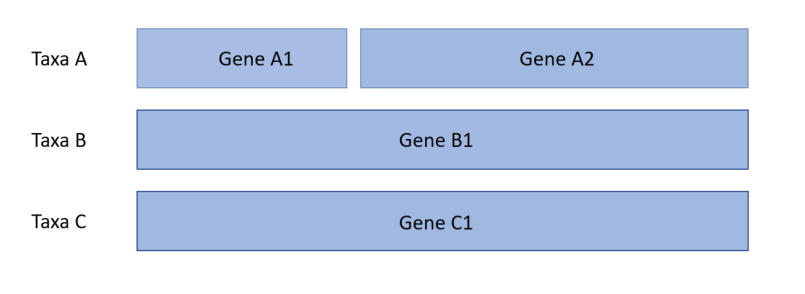
\includegraphics[width=\textwidth]{overlapgenes.png}\label{overlap}

\section*{Permutation Test}
I want to ensure that I understand the test correctly.
First, I create my new permuted blocks with the same number of genes as the original block length (i.e. if the block was composed of 2 genes, my permuted block will also contain 2 genes).
Second, I do a test (Wilcoxon?) to determine if the expression of the ATCC gene (which was inverted in the original block) is significantly different than the others. \textbf{Is this the test I should be doing?}
Third, I repeat the first two steps many many times.
Fourth, create a distribution of the p-values.
Fifth, see where my original p-value falls within that distribution.

\textbf{Is this general process correct?}

%\section*{Permutations: Gene expression}
%I did permutations tests shuffling gene expression and inversion status to see if the means differ between inverted and non-inverted regions. 
%I did this for all blocks, looking at the overall difference between inverted and non-inverted regions.
%The result was not significant (which is opposite from what the wilcoxon test said).
%I also did a permutation test on a per-strain basis and found no difference between inverted and non-inverted regions and genes for each strain (which is opposite from what the wilcoxon test said for ATCC).
%This to me means that generally there is no difference between inverted and non-inverted regions.
%But, on a gene level, we do see difference between some inverted genes (see below, and Wilcoxon tests per block).
%\textbf{Overall, do you think this is still worth stating? Or since we only have a small number of inverted genes that have a significant difference in expression (8\% of inverted genes), should I change the tone of the paper to say that inversions only seem to have some gene specific effects?}
%
%However, when I did a permutation test with just the non-inverted regions of ATCC and all other strains, the test was not significant.
%Indicating that the non-inverted regions of ATCC have no expression difference than non-inverted regions of other strains. 
%Which means that any difference we do see is not just due to ATCC but the inversions! Yay!
%
%I did not do a permutation test comparing inverted and non-inverted genes within each block (this would be hundreds of tests).
%\textbf{Do you think that I should do a permutation test per block? Is this too much? Can we just stick with the Wilcoxon test results per block?}
%
%
%
%\section*{Ancestral Inversion}
%I ran PARSNP on a few different close outgroups: \efer, \ecol Saki, \ecol K5198, \ecol TW. 
%The other strains are \ecoli K-12 MG1655, K-12 DH10B, BW25113 and ATCC 25922.
%\textbf{Do you think is is ``close'' enough as an outgroup choice for inversions?}
%
%I ran this analysis and here are the results:
%
%\textbf{\efer}
%\begin{itemize}
%	\item 17.7\% of blocks had outgroup = K-12 MG = ATCC
%	\item 31.8\% of blocks had outgroup = K-12 MG
%	\item 39.4\% of blocks had outgroup = ATCC
%	\item 11\% of blocks had the outgroup with a different sign than both ATCC and K-12 MG
%\end{itemize}
%
%\textbf{\ecol Saki}
%\begin{itemize}
%	\item 36.2\% of blocks had outgroup = K-12 MG = ATCC
%	\item 56.4\% of blocks had outgroup = K-12 MG
%	\item 5.1\% of blocks had outgroup = ATCC
%	\item 2.1\% of blocks had the outgroup with a different sign than both ATCC and K-12 MG
%\end{itemize}
%
%\textbf{\ecol K5198}
%\begin{itemize}
%	\item 32.4\% of blocks had outgroup = K-12 MG = ATCC
%	\item 31.3\% of blocks had outgroup = K-12 MG
%	\item 32.3\% of blocks had outgroup = ATCC
%	\item 3.9\% of blocks had the outgroup with a different sign than both ATCC and K-12 MG
%\end{itemize}
%
%\textbf{\ecol TW}
%\begin{itemize}
%	\item 4.3\% of blocks had outgroup = K-12 MG = ATCC
%	\item 7.8\% of blocks had outgroup = K-12 MG
%	\item 62.3\% of blocks had outgroup = ATCC
%	\item 25.5\% of blocks had the outgroup with a different sign than both ATCC and K-12 MG
%\end{itemize}
%
%Keep in mind that these blocks \textbf{are not} the same as the ones I am using in my analysis.
%So I am not sure what to do because depending on which strain is considered the ``outgroup'' it appears as though this ancestor is mostly similar to the K-12 MG strain or mostly similar to the ATCC strain.
%However, with each analysis, there are always some blocks that are in both categories (similar to MG or similar to ATCC).
%
%Even if we did choose one of these strains, the blocks are not the same as the ones I am using in my analysis. 
%Unfortunately, I think the correct thing to do is to do an actual reconstruction of each block (either sequence or character state) to determine what the ``inverted'' state should be.
%I found \uhref{http://www.phytools.org/eqg/Exercise_5.2/}{this website} that discusses how to use an R package called phytools to do character state reconstruction using .
%This might be a quicker and simpler option, rather than doing my long reconstruction method I used in the substitutions paper.
%
\end{document}
